\documentclass[10pt,letterpaper]{article}
\usepackage{tools}
\usepackage{enumitem}
%\settextfont{B Nazanin}
\usepackage{lipsum}
\setlength{\parskip}{3mm}
\setlength{\parindent}{0mm}
\newcommand{\wid}{0.49\textwidth}
\newcommand{\widone}{60mm}
\begin{document}
\Large
\begin{center}
In the name of beauty

5th problem set of ComNet course
\hl
\end{center}
Q1)

Determine the following statements as true or false. (Use enough reasons and explanation to support your answer)

\begin{enumerate}[label=\alph*-]
\item
The rdt 3.0 protocol is a special case of Go-Back-N protocol without pipelining (window size = 1).
\item
In GBN protocol, the window size has no relation with the number of bits in the packet sequence number field, however this is not the case in SR protocol.
\item
The sender sides of the FSMs of GBN and SR are the same.
\item
In the full-duplex transmission between two hosts, two TCP connections, one at each direction is needed.
\item
In a three-way handshaking, the first segment cannot carry any payload, though the other two can.
\end{enumerate}

Q2) A TCP connection is established between a sender and a receiver and segments with 250bytes of data are transmitted from the sender to the receiver. The initial sequence number is randomly chosen in the interval $[0,499]$bytes. Assume a flying, abandoned (!) packet with segment-number=289bytes and left from a previously brought-down TCP connection suddenly reaches the sender. What is the probability that the sender \underline{never regards} this packet as legitimate and bypasses it?

Q3)

Assume a sender transmits 4 segments back-to-back labeled from 0 to 3 to a receiver:
\newpage
\begin{figure}[htb]
\centering
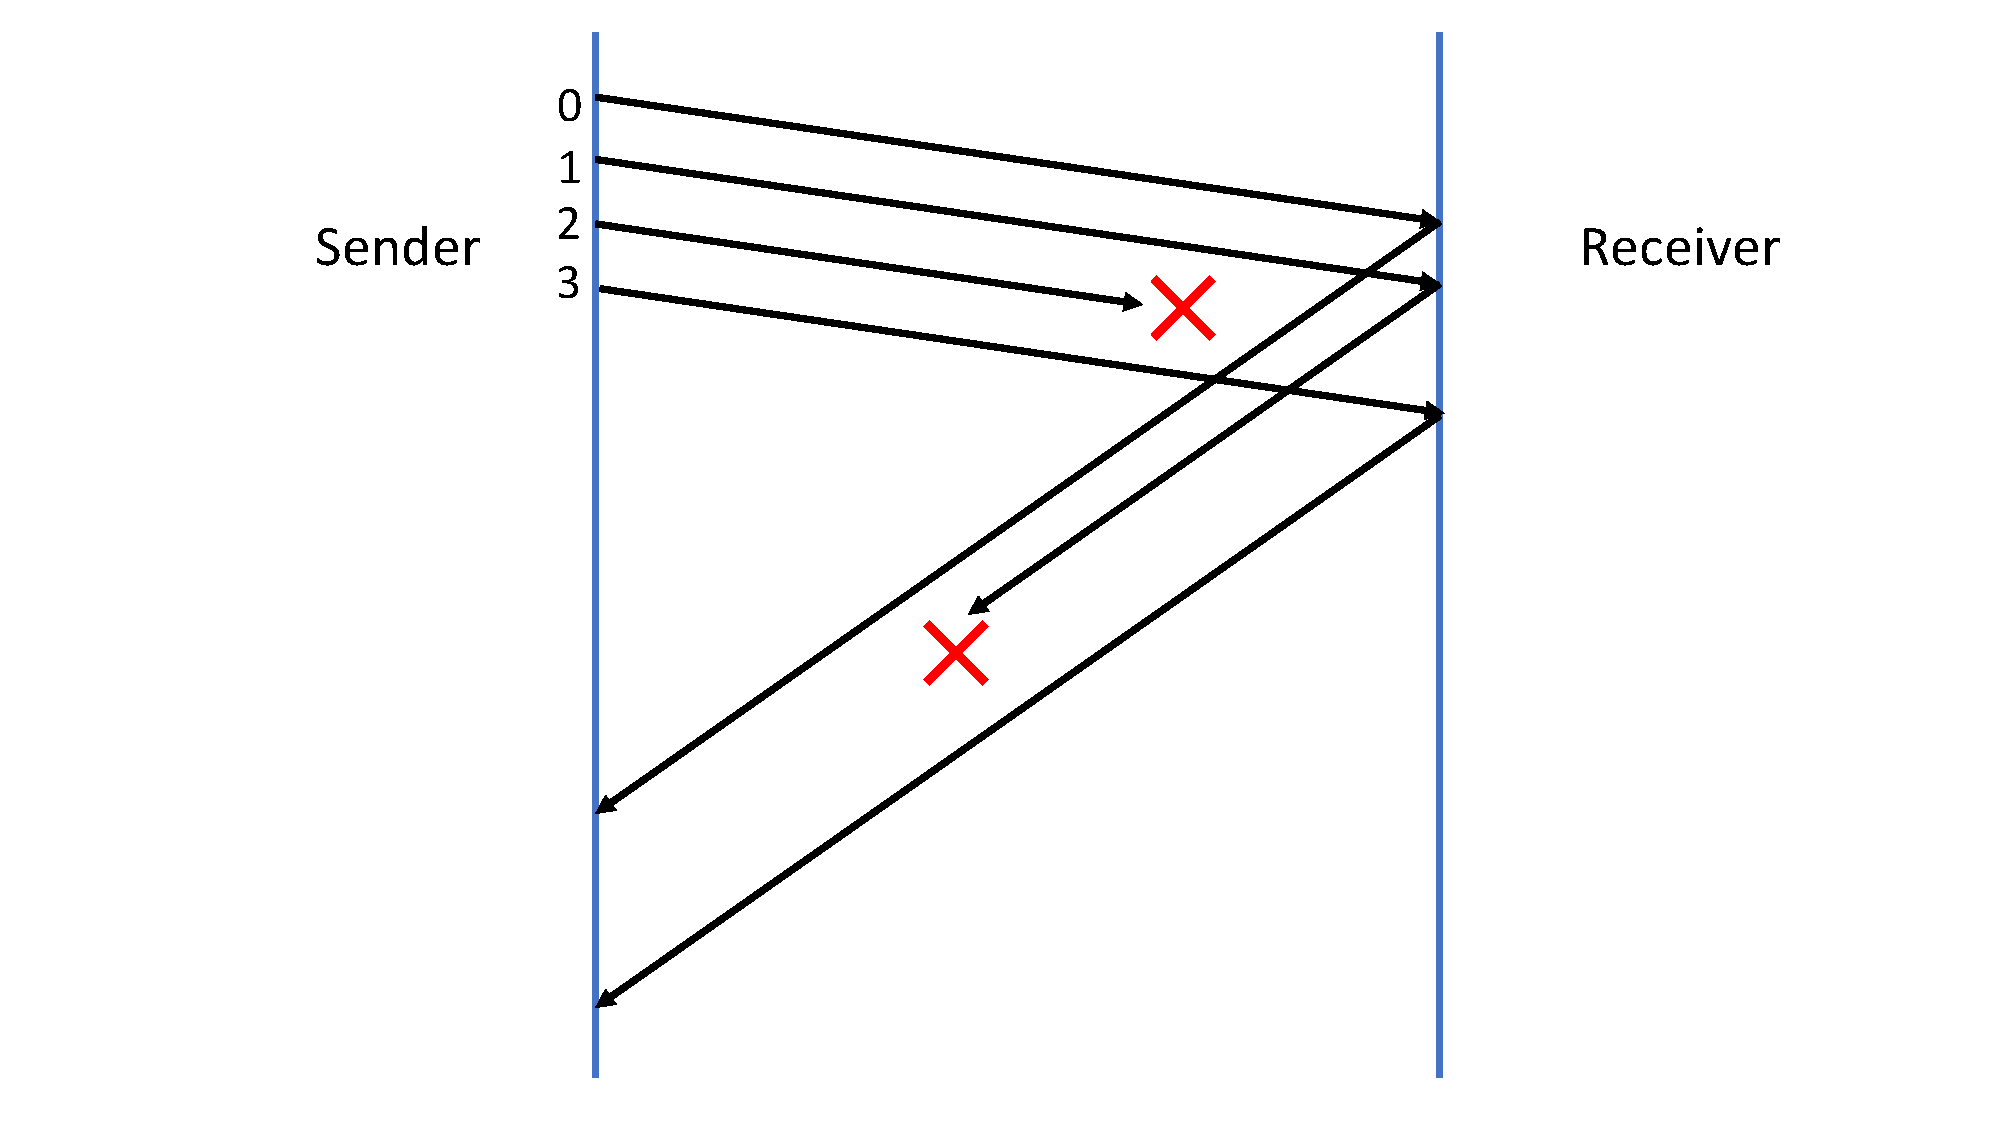
\includegraphics[width=100mm]{gbn_sr.pdf}
\caption{rdt2.1 sender}
\end{figure}

The packet numbered 2 does not make it all the way to the receiver and the packet numbered 1, is correctly received but the corresponding ACK does not reach the sender. Describe what operations would SR and GBN perform.

Q4) A GBN sender transmits 4 packets numbered from 0 to 3 to a receiver. Each packet is probable to be dropped in the intervening channel with a probability of $p$, but ACKs are never lost. Assume the transmission- and propagation delays of all the packets to be 0. If we denote the average number of transmission of packet $i$ to the receiver, until the first correct reception, by $n_i$, then find it for $i=0,1,2,3$.
%Determine the following statements as true or false with enough reasons.
%\begin{enumerate}[label=\alph*-]
%\item
%Both trasport and network layer protocols provide logical communication between processes running at different hosts rather than hosts themselves.
%\item
%Transport layer packets are refered to as \textbf{datagrams}.
%\item
%TCP ensures that the transmitted packets would finally reach their destination, however it makes no guarantee on the order of packets.
%\item
%The IP service model is a best-effort delivery service since it guarantees to deliver segments between communicating hosts, whether orderless or not.
%%\item
%%Cookies are used to keep track of user IDs in a stateless HTTP server.
%%\item
%%Link-layer switches are typically capable of processing the packets up to the layer 3.
%%\item
%%SMTP and FTP are examples of layer 1 protocols while TCP is a transport layer protocol.
%%\item
%%API is a set of rules 
%%\item
%%For economical reasons, exploiting optical fibers is not recommended in long-haul network
%\end{enumerate}
%
%Q2)
%\begin{enumerate}[label=\alph*-]
%\item
%Why is IP said to be an unreliable service and if so, how would TCP provide reliable data transfer on top of IP?
%\item
%Why are source and destination host port numbers included in segment headers? What problem could arise if they are ignored?
%\end{enumerate}
%
%Q3) Suppose Client A initiates a Telnet session with Server S. At about the same
%time, Client B also initiates a Telnet session with Server S. Provide possible
%source and destination port numbers for
%\begin{enumerate}[label=\alph*-]
%\item
%The segments sent from A to S.
%\item
%The segments sent from B to S.
%\item
%The segments sent from S to A.
%\item
%The segments sent from S to B.
%\item
%If A and B are different hosts, is it possible that the source port number in
%the segments from A to S is the same as that from B to S?
%\item
%How about if they are the same host?
%\end{enumerate}
%(Choose the port numbers at source and destination arbitrarily.)
%
%Q4) Consider the following Figure. What are the source and destination port values in the segments
%flowing from the server back to the clients’ processes? What are the IP
%addresses in the network-layer datagrams carrying the transport-layer segments?
%\begin{figure}[ht]
%\centering
%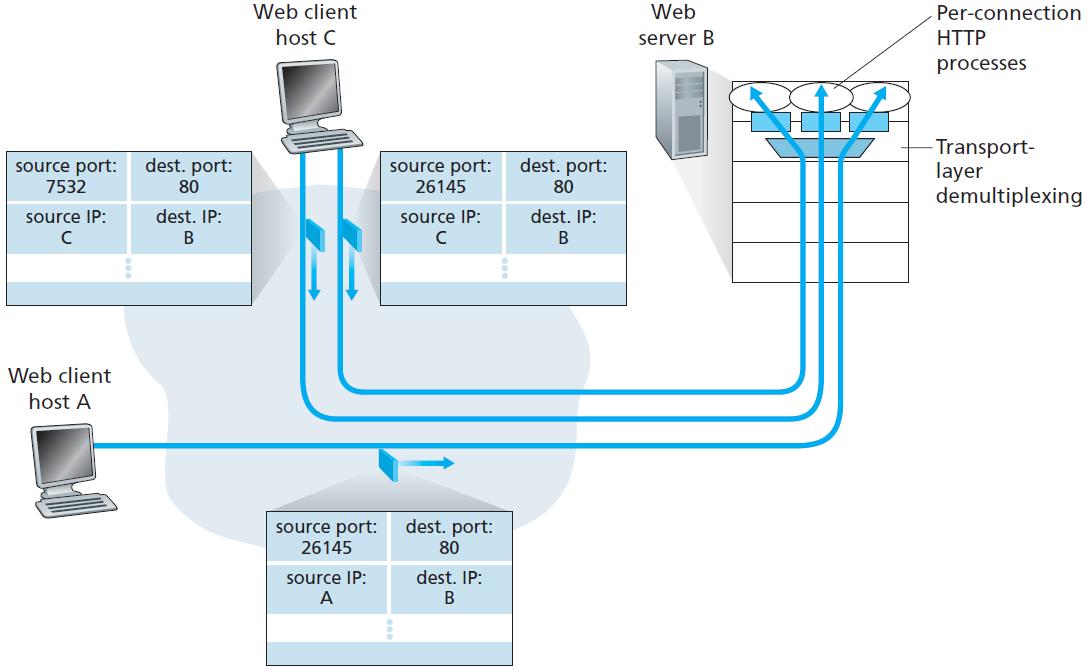
\includegraphics[width=180mm]{simnet}
%\end{figure}
\end{document}